\documentclass{article}
\usepackage{graphicx}
\usepackage{wrapfig}
\usepackage[skip=8pt,font=scriptsize]{caption}
\usepackage{subfig}
\usepackage{float}
\usepackage{fancyhdr}
\usepackage[letterpaper, portrait, margin=1.5in]{geometry}

\setlength{\parindent}{4em}
\setlength{\parskip}{0em}
\renewcommand{\baselinestretch}{1.15}
 
\pagestyle{fancy}
\fancyhf{}
\rhead{}
\lhead{}
\rfoot{Hasse Page \thepage}
\renewcommand{\headrulewidth}{0pt}

\begin{document}


\noindent 
Ariel Hasse\\
August 23, 2016\\
Summer Undergraduate Research Fellowship\\
Seven - Week Progress Report\\
California Institute of Technology\\
Professor David Hitlin’s Group\\



Over the past seven weeks I have continued to take data for my SURF research. As I mentioned in my last progress report I am determining the quenching factor for Barium Fluoride crystals. The quenching factor, also known as Birk's constant, describes the non-linear energy loss as particles varying by mass travel through the lattice of the crystal. This is important because $BaF_2$ is a scintillator, which are used in high energy physics experiments. When a particle collides with a scintillator it deposits energy, which excites an electron in the lattice. As the electron moves back to ground state it emits a photon and this continues through the scintillator. Barium fluoride is of particular interest because it has two mechanisms of scintillation, a fast and a slow component, which are at different wavelengths that determine how quickly photons are emitted. The fast component is at .6 nanoseconds, which provides many advantages, however presently it can not be separated from the slow component which scintillates at 620 nanoseconds. The ratios of energy from the fast and slow components from multiple photomultiplier tubes with varying quantum efficiency as a function of wavelength, determine the final quenching factor.  We find that the quenching factors can be determined from the ratios of the fast and slow components determined by the convolution. We measure the response of the $BaF_2$ crystal fast and slow components to alpha particles of known energies coming from the decay of slight radium contamination in the crystals. Confirmation with the known values allows for analysis of energy readout from gamma, electron, and alpha particles. In the past couple of weeks I have been finishing the data collection process so I can complete that analysis. 

I had three PMTs available for my research. In the first trial group I used the UV full spectrum extended PMT. This PMT can detect most light of wavelengths 150 to 450 nanometers with high light intensity [Figure 1]. Therefore the data collection process was relatively quick. I secondly attempted to take data with the XB2020 PMT. The XB2020 took over four days and did not have a good resolution for the fit [Figure 2]. We decided not to use this data and to instead use the first PMT with a shortpass filter. I next completed the data collection for the solarblind PMT which sees very little of the slow component light which constitutes most of the events. The radium measurement, the only alpha source, required 7 days to get enough counts to fit the peaks with a Gaussian. I am currently finishing data collection for the final set-up, the UV full spectrum extended with a short pass filter.


\begin{figure}[H]
  \centering
  \begin{minipage}[b]{0.4\textwidth}
    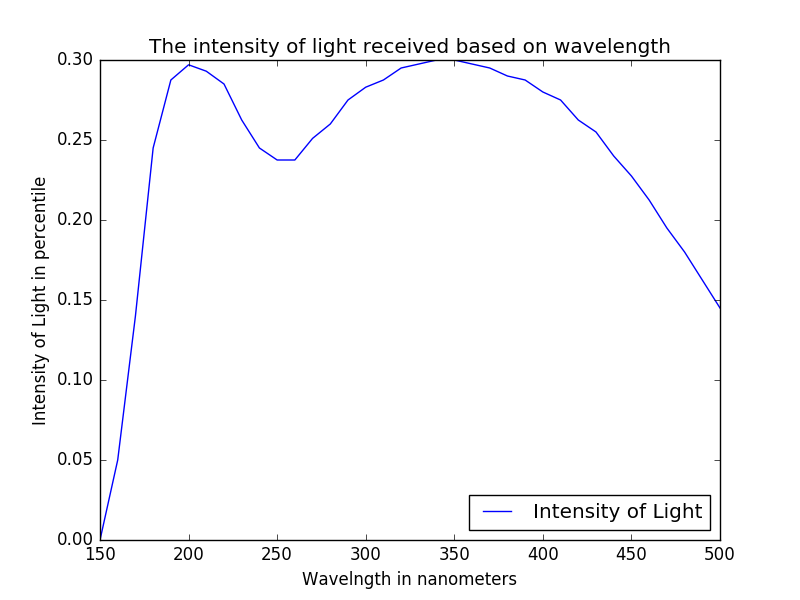
\includegraphics[width=\textwidth]{PMT1QE.png}
    \caption{UV Full Spectrum Extended PMT Quantum Efficiency}
  \end{minipage}
  \hfill
  \begin{minipage}[b]{0.4\textwidth}
    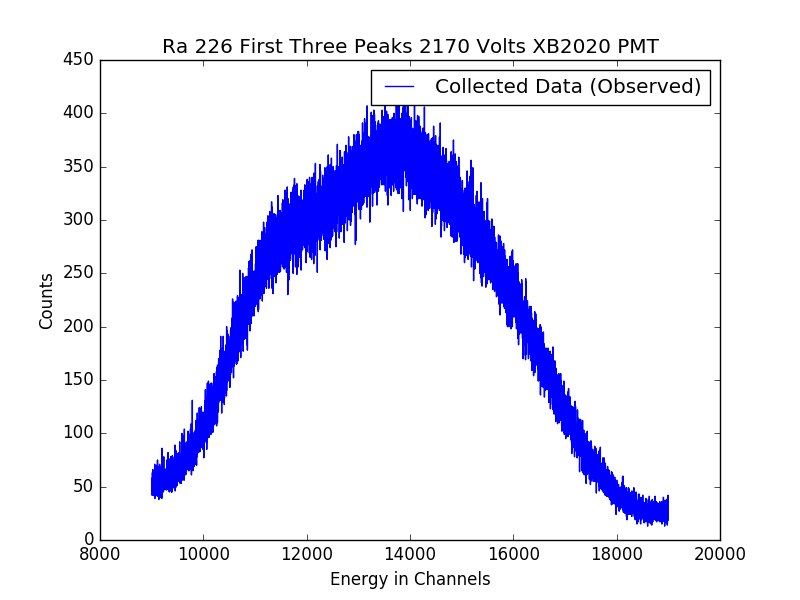
\includegraphics[width=\textwidth]{xb2020.png}
    \caption{XB2020 PMT Radium 226 First Three Peaks}
  \end{minipage}
\end{figure}


Once I have finished collecting data and fitting the energy peaks I will separate the slow and fast components for each set-up. I first convolve the emission spectrum for $BaF_2$ with the quantum efficiency for the PMT. The area under the first two Gaussians represents the portion of light from the fast component. The third hump is a function composed from two Gaussians and the area under that curve represents the light from the slow component [Figure 3]. These proportions create a linear function for that PMT. The intersection of the linear function for each PMT provides the ratio for both the fast and slow components for that energy level. I will complete this for each of the four radium peaks to create an energy dependent function that describes the quenching factor for the fast and slow components for alpha particles with Barium Fluoride crystals.

\begin{figure}[H]
  \centering
  \begin{minipage}[b]{0.4\textwidth}
    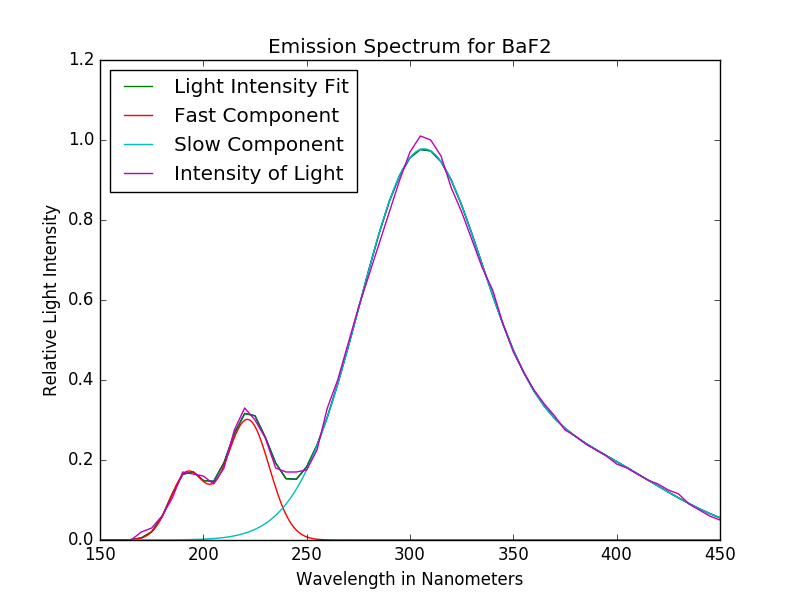
\includegraphics[width=\textwidth]{FitsBaF2.png}
    \caption{The black line is the convolution of the quantum efficiency of the PMT and the emisison spectrum for $BaF_2$ }
  \end{minipage}
\end{figure}

I also improved my variable control for data collection. The PMTs are affected by temperature. For this purpose we leave the PMT powered at all times to maintain a steady state. However the laboratory temperature is uncontrollable. I fitted a temperature sensor system in the lab to record the temperature while I am not there. It is an arduino circuit board, which can be fitted for many probes. I wrote a program in the arduino language for this purpose. I also wrote a python script to analyze the output to determine the deviation in temperature. Beyond the practical use in my research the probe may be useful in future experiments and the skills I acquired will certainly help me. 

To further improve my computer programming skills and to make my work more accessible I also created a github account and jupyter notebooks. Now my code is stored online and the jupyter notebook interface allows me to generate figures in the working code. All of my code and other works related are now in a git repository on my computer and can be pushed to an online github for storage and viewing. My work is now better documented, more accessible, and secure. 

In the final weeks of my project I will finish data collection and analysis as described above and in previous reports. I don't anticipate any challenges in the laboratory, however I am prepared for issues in the analysis pipeline. Since I converted to jupyter notebooks, I am still finding processing errors that will have to be dealt with. I should be able to run everything smoothly, but I also have several people in my group to assist me. After compiling all of my results I will lastly explore the physical mechanisms behind this phenomena.



\setlength{\parskip}{2em}
\noindent
Bibliography

\noindent
Birks, J.B. (1964). The Theory and Practice of Scintillation Counting. London:
Pergamon.

\noindent
Polischuk, O., Belli, P., Bernabei, R., Capella, F., Caracciolo, V., Cerulli, R., . . . Tretyak, V. (2009). Radioactive contamination of BaF2 crystal scintillator. Nuclear Institute.


\end{document} 
